\chapter{Vorstudie}\label{Vorstudie}
Um zu erproben, wie digitale Türschilder funktionieren und wie sie von Studenten und Mitarbeitern der Medienfakultät der Bauhaus Universität Weimar aufgenommen werden habe ich die Entscheidung getroffen ein bereits vorhandenes Projekt herzunehmen und damit eine Anforderungsanalyse durchzuführen.
Dafür wurde die zweite Version des NetBoards Projekts\cite{netboards:website} auf einem privaten Server aufgesetzt.
\section{NetBoards Experiment}\label{NetBoards Experiment}
%\cite{apache:website}
%\cite{python:website}
Als Grundlage für meinen Experiment diente ein virtueller Debian-Linux Server mit 1,5GHz AMD CPU und 2GB RAM auf dem Apache2 als Webserver und Python2 für serverseitige Scripts liefen. Das öffentlich zugängliche NetBoards2 Projekt wurde installiert und konfiguriert.\\
Nachdem der Server eingerichtet war kam die Frage auf, was als Anzeigegerät dienen sollte. Das originale Projekt von E. Wood wurde für 22 Zoll Monitore mit Touch-Oberfläche entworfen. Diese wurden vertikal neben die Büroeingänge gehangen.\\
Da für mein Experiment nicht die notwendigen Ressourcen vorhanden waren, um den genauen Versuchsaufbau nachzuempfinden, fiel die Wahl des Anzeigegerätes auf einen kostengünstigen Tablet-PC.
\\
\todotext{was war das nochmal für ein tablet? 10Zoll? Spezifikationen angeben}\\
Damit die Benutzer nicht mit den auf dem Gerät installierten Applikationen interagieren konnten wurde eine Kiosk-Applikation installiert.
Diese App schränkt die Interaktionsmöglichkeiten der Nutzer nur auf eine ausgewählte Webseite ein. Nur der Administrator des Gerätes hat die Möglichkeit diese zu ändern oder die Applikation ganz zu beenden.\\
Ein weiteres Problem war die Befestigung des Displays.
Ich entschied mich dafür, das Tablet an den bereits vorhanden Türschildern anzubringen (Abb. \ref{img:tuerschild}).
\begin{figure}[h!]
  \centering
    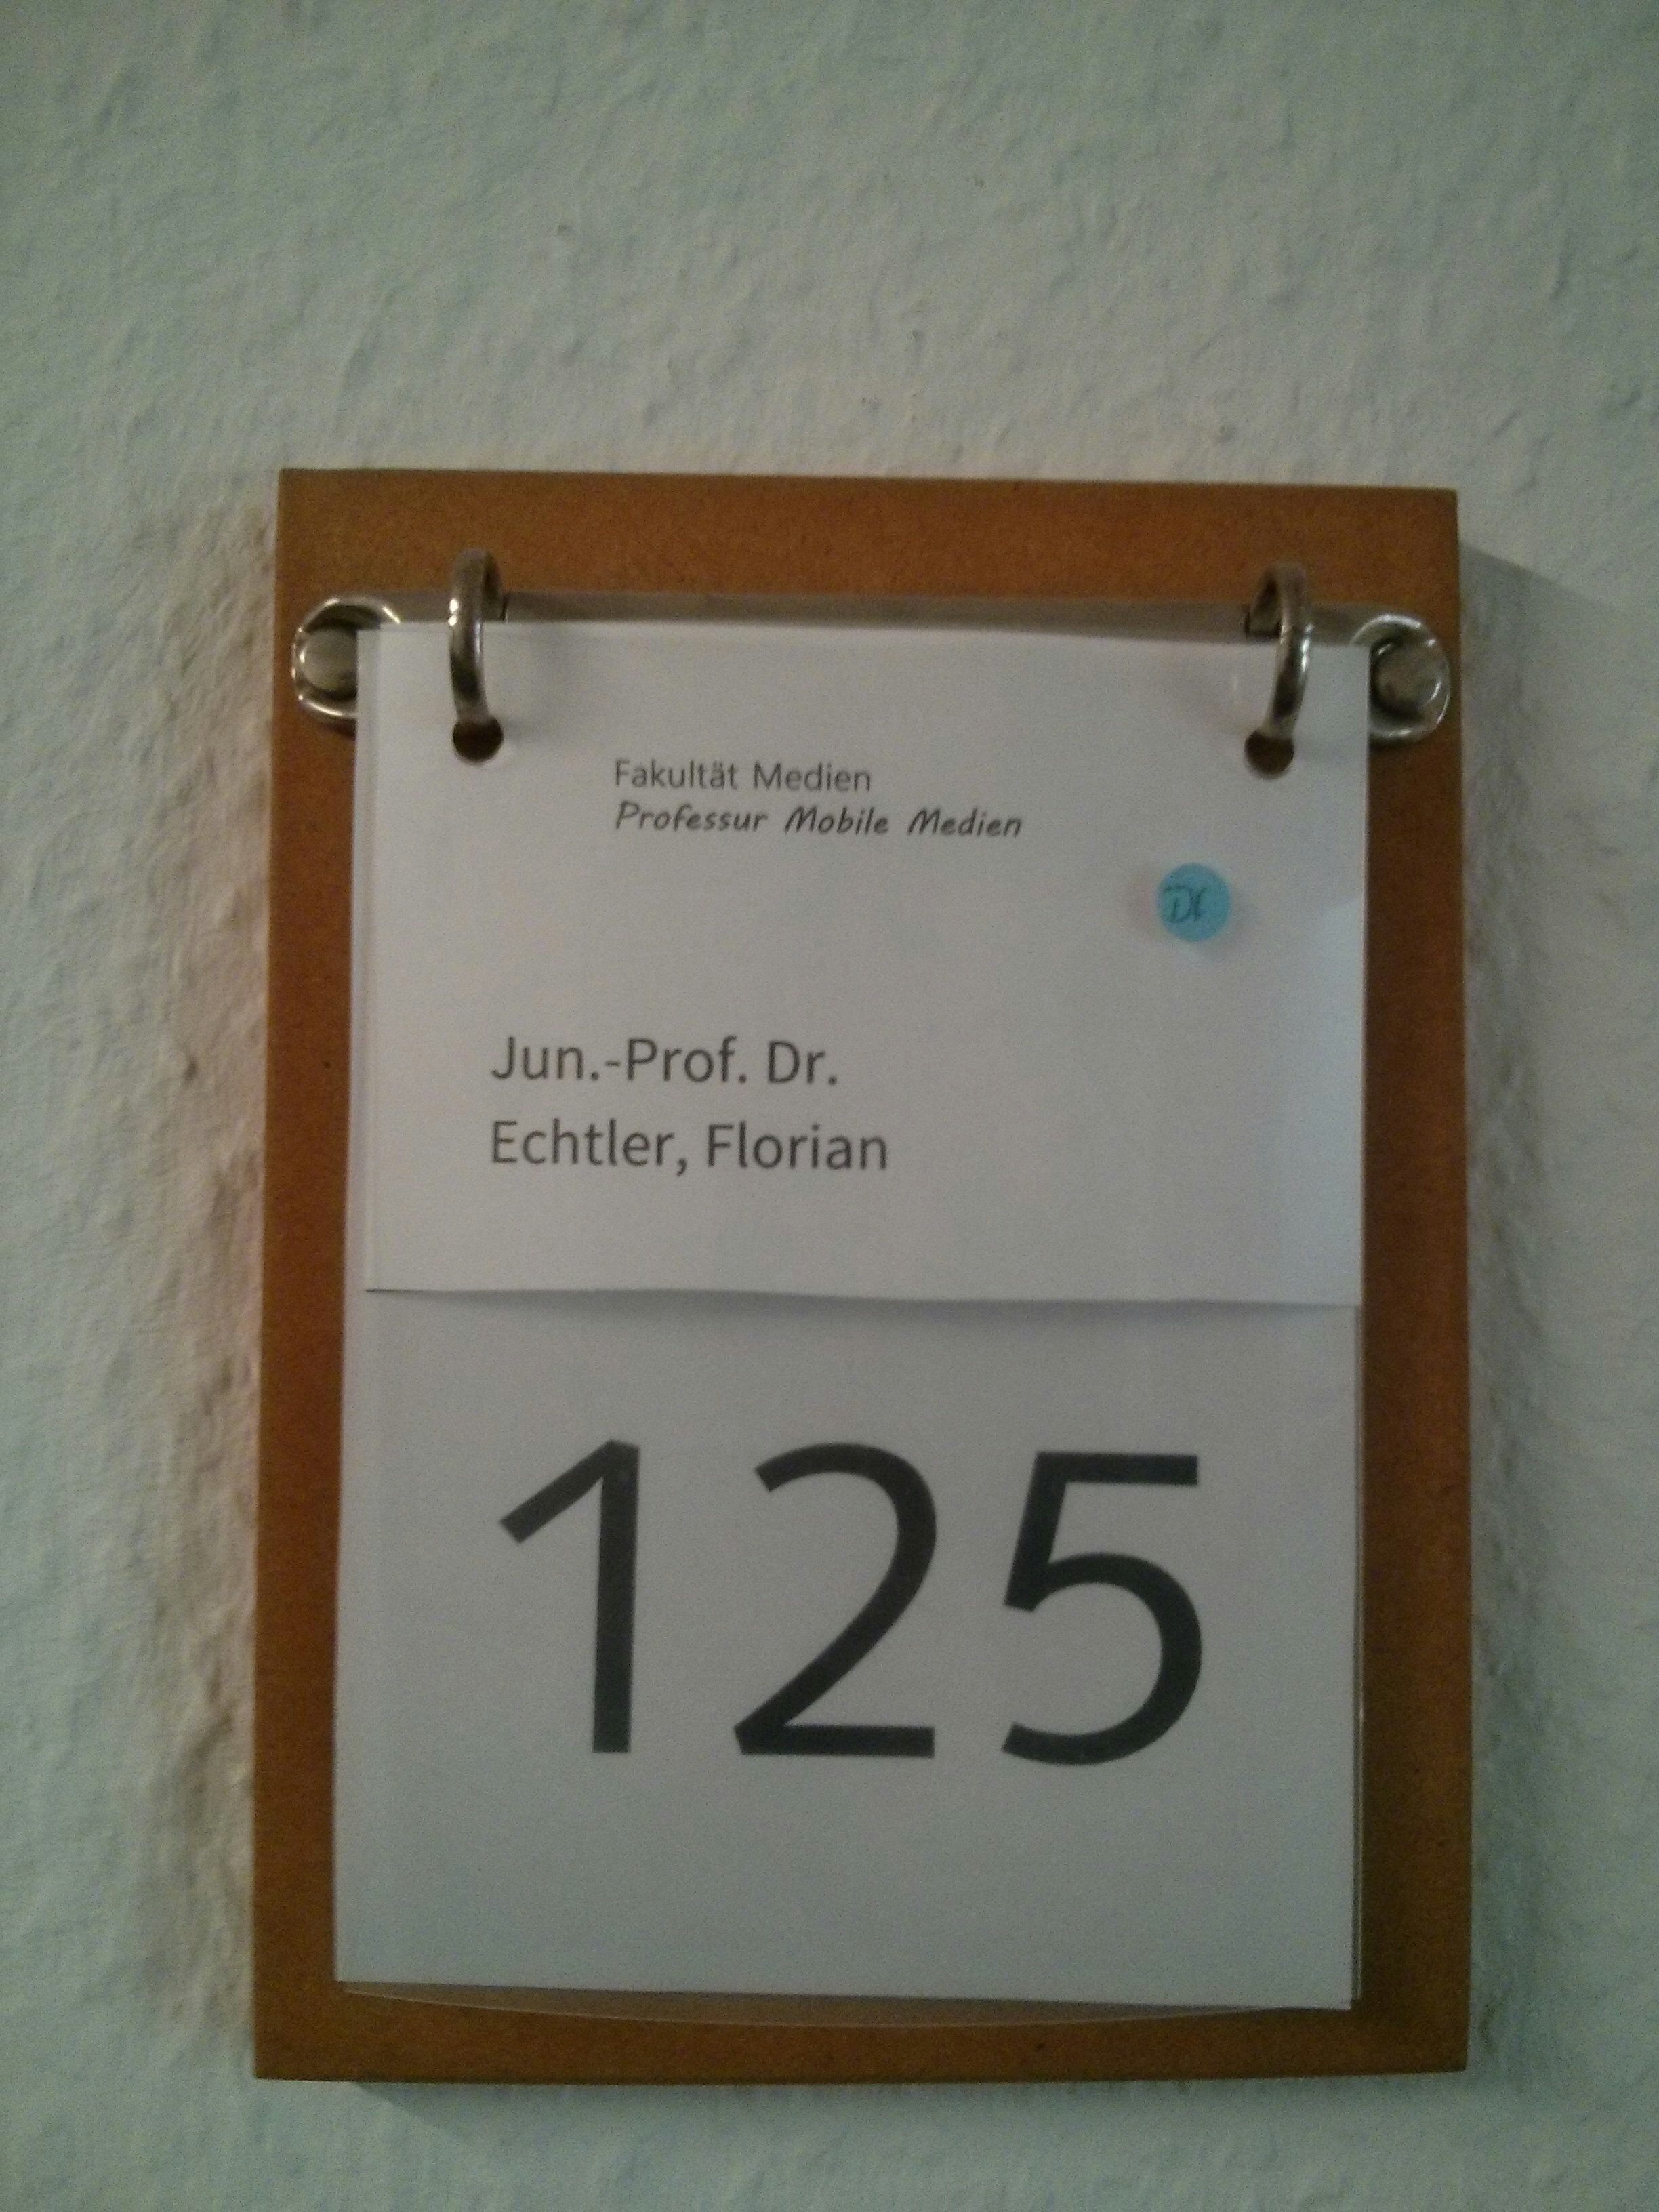
\includegraphics[width=0.5\textwidth]{./img/Tuerschild.jpg}
  \caption{Ein typisches Türschild in der Medienfakultät}
  \label{img:tuerschild}
\end{figure}\\
Dadurch, da sich die Rückwand des Tablets abschrauben ließ konnte ich zwei Löcher hinein bohren. Diese dienten zur Anbringung eines Drahtes, welcher über das Türschild gehangen werden konnte. Für dieses Experiment war die Aufhängung vollkommen ausreichend.\\
Für die Stromversorgung wurde das Ladekabel des Tablets verlängert, damit es an eine Steckdose im Büro angeschlossen werden konnte.\\
Als Testnutzer für das Experiment konnte ich zwei Mitarbeiter der Professur für Webtechnologien und Informationssysteme organisieren.
Diese Nutzer teilten sich ein Büro, wodurch nur ein Anzeigegerät benötigt wurde. Nach einer Einweisung zur Benutzung des Systems wurde klar, dass die zwei Tester nicht damit einverstanden waren, dass durch die Interaktivität des Boards jeder vorbeigehende Gast den dargestellten Inhalt nach belieben ändern konnte. Es hätte sein können, da durch die Anonymität der Gäste, das Board missbraucht werden könnte, um unangebrachte Skizzen zu zeichnen.
Aus diesem Grund habe ich für die Nutzer zwei verschiedene Ansichten erstellt:
\begin{itemize}
  \item Eine Backend-Sicht, auf der die Tester ihre Änderungen machen konnten.
  \item Eine Frontend-Sicht, die auf dem Tablet angezeigt wurde, nach 5 Minuten den aktuellen Stand abspeicherte und die Sicht auf den aktuellsten Stand der Backend-Sicht setzte.
\end{itemize}
\begin{figure}[h!]
  \centering
    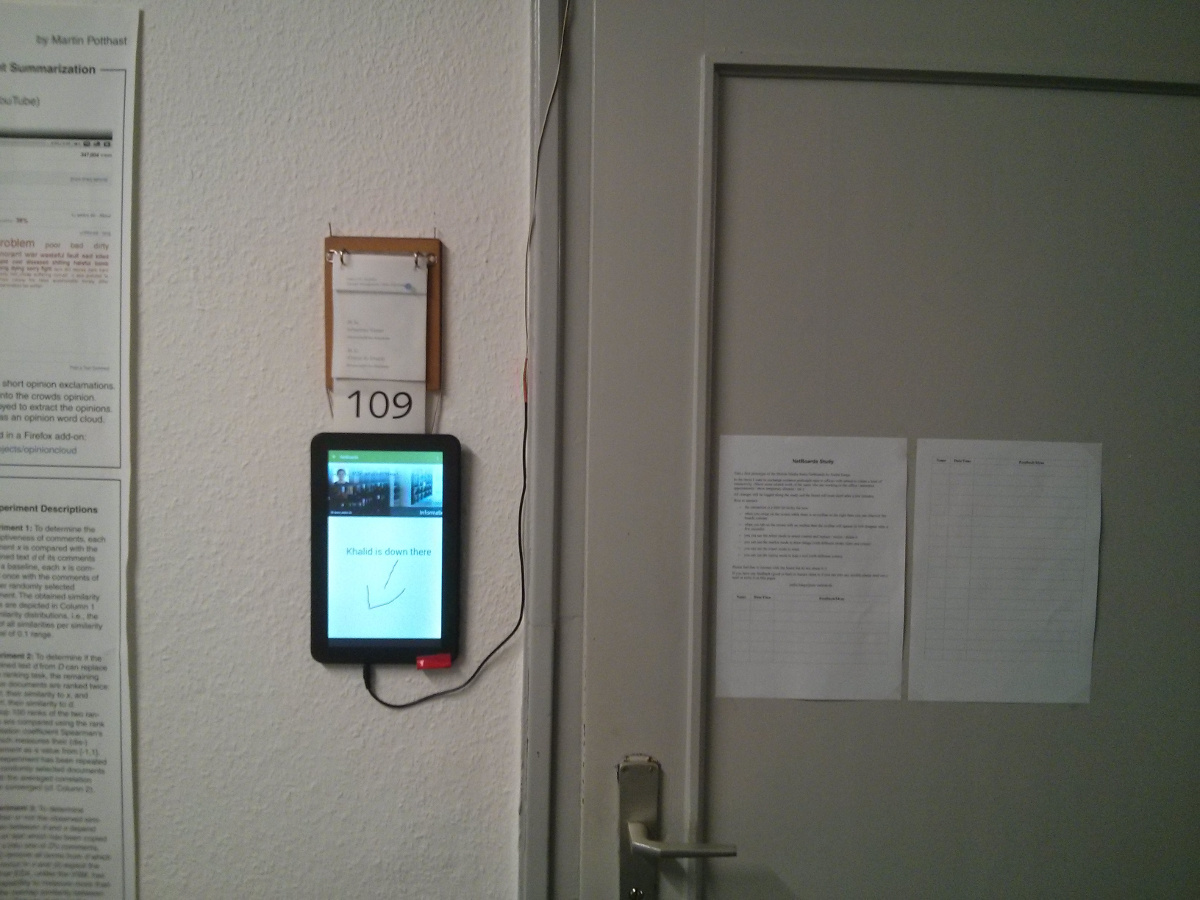
\includegraphics[width=0.7\textwidth]{./img/experiment01.jpg}
  \caption{Versuchsaufbau des Experiments}
  \label{img:experiment01}
\end{figure}



% Experiment Dauer
% 28.05.2015 - 08.06.2015
% 12 Tage
\section{Auswertung}\label{Auswertung}
Das Experiment lief 12 Tage. Die Nutzer erstellten sich zu Beginn einen Nutzeraccount und richteten ihr Board ein (Abb. \ref{img:experiment02}). Jeder der beiden lud ein Profilbild hoch und gab seinen Namen, sowie seinen akademischen Grad an.
Einer der Tester benutzte das Display um das Banner der Professur zu präsentieren und um Gäste beispielsweise darüber zu informieren, dass er sich zur Zeit im Büro befindet (Abb. \ref{img:experiment03}).\\
Sehr erfreudig war, dass das Board viel Aufmerksamkeit zu erzeugen schien. Viele vorbeigehende Nutzer blieben stehen, um sich das Display genauer anzusehen und interagierten sogar damit. Dadurch entstanden viele Zeichnungen, wovon viele keinen tieferen Sinn hatten wie Beispielsweise die Zeichnung in Abb. \ref{img:experiment04}. Jedoch gab es auch ab und an Nachrichten, die direkt an die Besitzer des Boards gerichtet waren, wie das Bild einer Kaffeetasse mit einem Fragezeichen aus Abb. \ref{img:experiment05}, was die Frage nach einer Kaffeepause darstellen sollte.
\begin{figure}[]
  \centering
    \subfigure[erste Änderung der Nutzer]{
      \frame{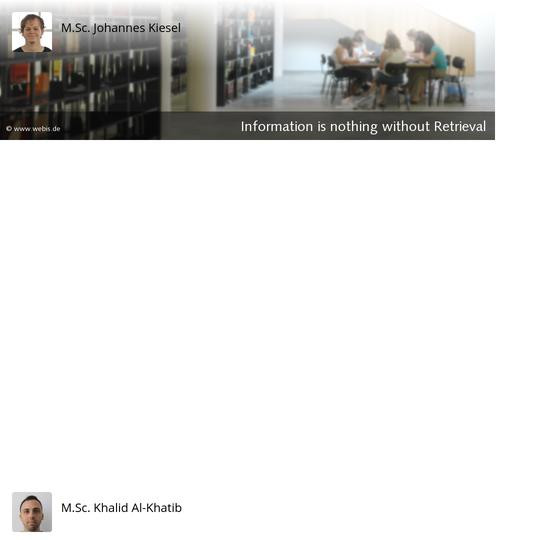
\includegraphics[width=0.35\textwidth]{./img/experiment02_empty.jpg}}
      \label{img:experiment02}
    }
    \subfigure[Statusangabe eines Nutzers]{
      \frame{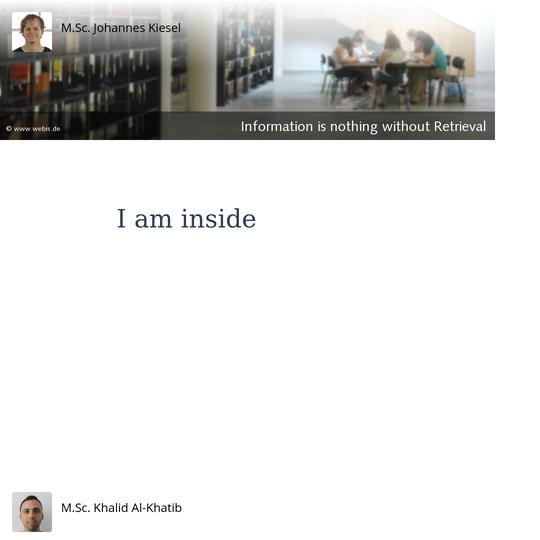
\includegraphics[width=0.35\textwidth]{./img/experiment03_statusContent.jpg}}
      \label{img:experiment03}
    }
    \subfigure[gezeichnetes Bild eines Gastes]{
      \frame{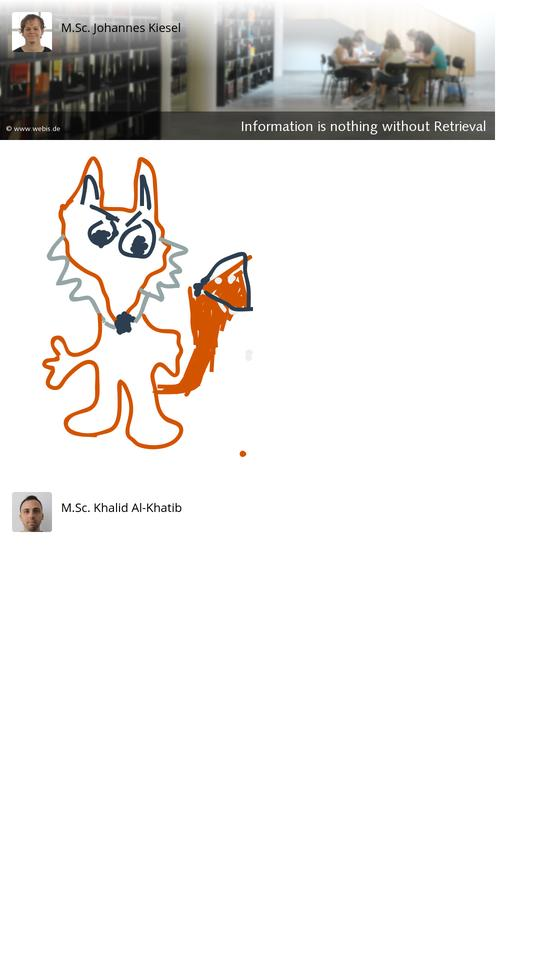
\includegraphics[width=0.35\textwidth]{./img/experiment04_fox.jpg}}
      \label{img:experiment04}
    }
    \subfigure[Frage eines Gastes]{
      \frame{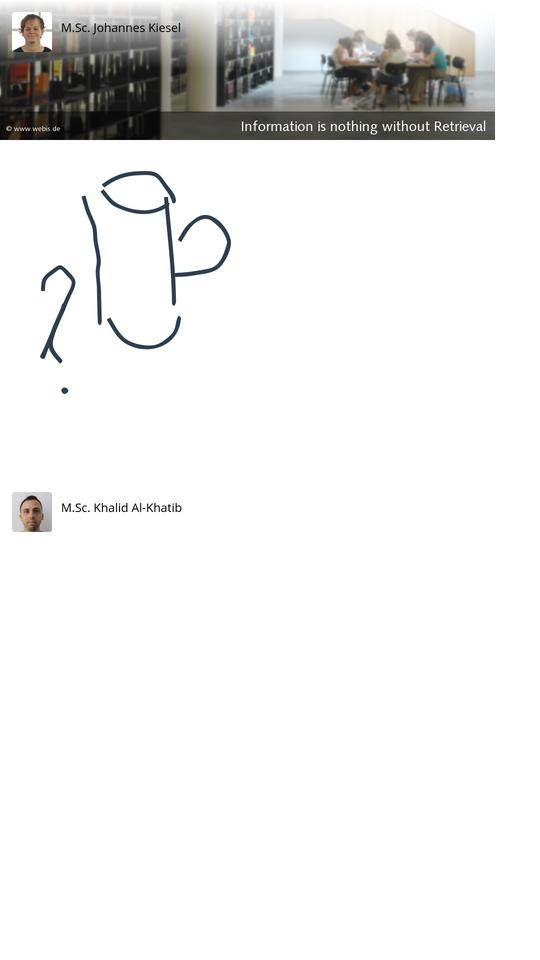
\includegraphics[width=0.35\textwidth]{./img/experiment05_coffee.jpg}}
      \label{img:experiment05}
    }
  \caption{Einige Beispielbilder}
\end{figure}
Nachdem das Experiment beendet war
%Egebnis:
%- Durch zu geringe Tabletauflösung war den meisten Nutzern nicht bewusst, dass 2 Leute in dem Raum sind
%- Scrolling war nur möglich, wenn der Sidebar weg war, was die meisten Nutzer nicht wussten - hängt auch mit der Auflösung zusammen, da %Widescreen Monitor im Portrait Modus bei Netboards genutzt wurde
%- Durch schlechte Tablet Hardware war die Interaktion sehr langsam und hat äußerst stark gelaggt
%- Statusmeldungen wie "I am inside wurden sehr gut aufgenommen", da Nutzer dadurch wussten, dass der Nutzer zur Zeit im Raum ist, ohne zu Klopfen
%- Die Nutzer im Raum haben nicht mitbekommen, wenn jemand etwas auf ihr Board geschrieben haben - Da das Plugin nicht installiert wurde
%- ein/zwei Bilder, die gezeichnet wurden
%- Dem Nutzer war nicht genau klar, wofür er das Tool benutzen sollte
%- Abusing durch die implementation eines shared displays im pseudo privaten bereich vor büros: jeder konnte etwas ändern und die Besitzer der Boards hatten nicht immer die möglichkeit zu überprüfen, was geändert wurde, wodurch es viele unangebrachte Skizzen gab.
%Besitzer sowie Besucher konnten den Inhalt, der auf dem Display angezeigt wurde ändern, wodurch jedem Benutzer direkt in den präsentierten Inhalt eingreifen konnte. (Eben genau so wie ein öffentliches Whiteboard, wo jeder der vorbei geht etwas ändern kann)  -- hier könnte ich vllt auch das beispiel der mensa whiteboards bringen ---- Kinderhacksteak anstelle vom Rinderhacksteak


